\documentclass[tikz]{standalone}
%\documentclass{article}
\usepackage{tikz}
\usepackage{amsmath}
\begin{document}
  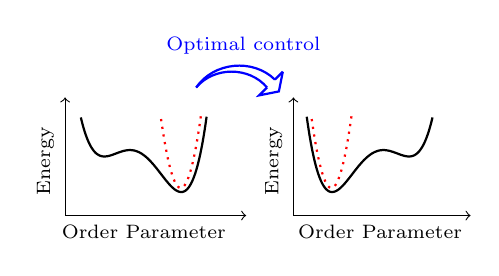
\begin{tikzpicture}[domain=-0.3:1.3] 
    %\draw[very thin,color=gray] (-0.1,-1.1) grid (3.9,3.9);
    \draw[->] (-0.5,4.25) -- (1.8,4.25) node[below] at (0.5,4.25) {\scriptsize{Order Parameter}}; 
    \draw[->] (-0.5,4.25) -- (-0.5,5.75) node[left,rotate=90] at (-0.75,5.5) {\scriptsize{Energy}};
    \draw[->] (2.4,4.25) -- (4.65,4.25) node[below] at (3.5,4.25) {\scriptsize{Order Parameter}}; 
    \draw[->] (2.4,4.25) -- (2.4,5.75) node[left,rotate=90] at (2.15,5.5) {\scriptsize{Energy}};
    %\draw[->] (4.25,9.25) -- (4.25,10.75) node[left,rotate=90] at (4.1,10.75) {\scriptsize{Energy}};
    %\draw[color=red]    plot (\x,\x)             node[right] {$f(x) =x$}; 
    %\draw[blue] plot (\x,{sin(\x r)})    node[right] {$f(x) = \sin x$}; 
    %\draw[color=orange] plot (\x,{0.05*exp(\x)}) node[right] {$f(x) = \frac{1}{20} \mathrm e^x$};
    %\draw[color=red] plot (\x,{\x^6-5.5*\x^4+5*\x^2+10})
    %\samplesize{1000}
    %\draw[black,samples=200,thick] plot (\x,{(\x)^4 - 0.5*(\x)^3 + (\x)^2});
    \draw[black,samples=200,thick] plot (\x,{20*((\x)^4/4.5 - (\x)^3/2.6 + 0.14*(\x)^2) + 5.0});
    \begin{scope}[xshift=27]
    \draw[dotted,red,samples=200,thick, domain=-0.23:0.28] plot (\x,{14*((\x-0.02)^2)+4.6});
    \end{scope}
    \begin{scope}[xscale=-1, xshift=-110]
    \draw[black,samples=200,thick] plot (\x,{20*((\x)^4/4.5 -(\x)^3/2.6 + 0.14*(\x)^2) + 5.0});
    \end{scope}
    \begin{scope}[xshift=82]
    \draw[dotted,red,samples=200,thick, domain=-0.25:0.26] plot (\x,{14*((\x)^2)+4.60});
    \end{scope}
    %\draw[thick,blue] (-1.25,10) circle(0.2);
    %\draw [<->,thick,red] (-1,11) arc (180:45:18pt); 
    \begin{scope}[xshift=-1,yshift=5]
    %\draw[-latex,blue,thick] (0.0,5.8) to[out=50,in=135] (2.6,5.8) ;
    %\draw[-latex,red] (0.3,9.8) to[out=135,in=30] (-0.7,10.1) ;
    %\draw[-latex,red] (1.15,10.25) to[out=120,in=15] (0.1,10.8) ;
    %\draw[-latex,red] (0.15,10.75) to[out=15,in=120] (1.1,10.2) ;
    \draw[blue, thick] (2.3,5.9)--(2.25,5.65)--(2.0,5.6)--(2.10,5.70)coordinate(B);
	\draw[blue, thick] (2.3,5.9)--(2.2,5.8)coordinate(A);
	\path(A)  edge [thick, blue, bend right=50](1.2,5.7) node[above, blue] at (1.8,6.0) {\scriptsize{Optimal control}}; 
	\path(B)  edge [thick, blue, bend right=50](1.2,5.7);
    \end{scope}
    
  \end{tikzpicture}
\end{document}